%%%%%%%%%%%%%%%%%%%%%%%%%%%%%%%%%%%%%%%%%%%%%%%%%%%%%%%%%%%%%%%%%%%%%%%%
% RAPPORT DE PROJET zz2 2015-2016
% projet : Conception et mise en fonction d'une base de données pour la
%           représentation et l'utilisation des résultats d'un ou
%           plusieurs algorithmes de comparaison (dans le cadre du
%           projet LSST)
% tuteur : Bogdan Vulpescu (vulpescu@clermont.in2p3.fr)
% auteur : Josselin Massot (massot@poste.isima.fr)
%%%%%%%%%%%%%%%%%%%%%%%%%%%%%%%%%%%%%%%%%%%%%%%%%%%%%%%%%%%%%%%%%%%%%%%%


\documentclass[a4paper, 11pt]{article}

% -------------------------------------------------------------------- %
%                                                                      %
% fichier de préambule                                                 %
%                                                                      %
% Importantion de nombreux packages, plus francisation                 %
%                                                                      %
% -------------------------------------------------------------------- %

% ----------------------------------------------------------------------
% gestion du français, et des accents
\usepackage{cmap}
\usepackage[T1]{fontenc}
\usepackage[english,frenchb]{babel}
\usepackage[utf8x]{inputenc}
\usepackage{helvet}
\usepackage{courier}
%\renewcommand{\familydefault}{\sfdefault}
%\pdfcompresslevel=3


\usepackage{color}
\usepackage[table]{xcolor}

\usepackage{sectsty}
\allsectionsfont{\bfseries\sffamily\color{black!90}\hspace{-1em}}
\partfont{\sffamily}
\usepackage[font={small,it}]{caption}
\makeatletter
\def\@seccntformat#1{\llap{\csname the#1\endcsname\quad}}
\makeatletter\pdfcompresslevel=9
\def\@seccntformat#1{\llap{\csname the#1\endcsname\quad}}
\makeatother

% ----------------------------------------------------------------------
% packages pour les figures
\usepackage{graphicx}
\usepackage{subfig}
\usepackage{tikz}

% change la numéroration des figures
%%%% debut macro %%%%
\makeatletter
\renewcommand{\thefigure}{\ifnum \c@section>\z@ \thesection.\fi
 \@arabic\c@figure}
\@addtoreset{figure}{section}
\makeatother
%%%% fin macro %%%%

% change la numéroration des tableaux
%%%% debut macro %%%%
\makeatletter
\renewcommand{\thetable}{\ifnum \c@section>\z@ \thesection.\fi
 \@arabic\c@table}
\@addtoreset{table}{section}
\makeatother
%%%% fin macro %%%%

% ----------------------------------------------------------------------
% diagramme de Gantt
\usepackage{model/pgfgantt}

% ----------------------------------------------------------------------
% pour mettre une page en mode paysage
\usepackage{lscape}

% ----------------------------------------------------------------------
% Miscelianous
\usepackage[pdfborder={0 0 0 [3 3]}]{hyperref}
\usepackage{bookmark}

% ----------------------------------------------------------------------
%packages pour les maths
\usepackage{amsmath}
\usepackage{amssymb}
%\usepackage{amsfonts}
\usepackage{mathrsfs}
\usepackage{wasysym}
\usepackage{textcomp}
%\usepackage{bbm}

% ----------------------------------------------------------------------
% packages pour les algorithmes
\usepackage[section]{algorithm}
\usepackage[noend]{algpseudocode}

% francisation des algorithmes
\floatname{algorithm}{Algorithme}

\renewcommand{\algorithmicprocedure} {{\footnotesize \textbf{\textsf{Proc\'edure}} }}
\renewcommand{\algorithmicwhile}     {{\footnotesize \textbf{\textsf{Tant que}}    }}
\renewcommand{\algorithmicdo}        {{\footnotesize \textbf{\textsf{Faire}}       }}
\renewcommand{\algorithmicend}       {{\footnotesize \textbf{\textsf{Fin}}         }}
\renewcommand{\algorithmicif}        {{\footnotesize \textbf{\textsf{Si}}          }}
\renewcommand{\algorithmicelse}      {{\footnotesize \textbf{\textsf{Sinon}}       }}
\renewcommand{\algorithmicthen}      {{\footnotesize \textbf{\textsf{Alors}}       }}
\renewcommand{\algorithmicfor}       {{\footnotesize \textbf{\textsf{Pour}}        }}
\renewcommand{\algorithmicforall}    {{\footnotesize \textbf{\textsf{Pour tout}}   }}
\renewcommand{\algorithmicdo}        {{\footnotesize \textbf{\textsf{Faire}}       }}
\renewcommand{\algorithmicrepeat}    {{\footnotesize \textbf{\textsf{Répéter}}     }}
\renewcommand{\algorithmicuntil}     {{\footnotesize \textbf{\textsf{Jusqu'à}}     }}
\renewcommand{\algorithmicfunction}  {{\footnotesize \textbf{\textsf{Fonction}}    }}
\renewcommand{\algorithmicreturn}    {{\footnotesize \textbf{\textsf{Retourner}}   }}
\let\mylistof\listof
\renewcommand\listof[2]{\mylistof{algorithm}{Liste des algorithmes}}
\makeatletter
\providecommand*{\toclevel@algorithm}{0}
\makeatother
% Lister les algorithmes :
%\listofalgorithms % même principe que toc
\addto\captionsfrench{%
  \renewcommand{\listfigurename}{Liste des figures}%
}
\addto\captionsfrench{\def\figurename{Figure}}
\addto\captionsfrench{\def\tablename{Tableau}}

% ----------------------------------------------------------------------
% tableaux
\definecolor{tablegray}{gray}{0.9}%table

% ----------------------------------------------------------------------
% importantion de code
\definecolor{mygray}{rgb}{0.5,0.5,0.5} % définition du gris (n° ligne)
\usepackage{listings}
\usepackage{listingsutf8}
%%%%%%%%%%%%%%%%%%\renewcommand{\thelstlisting}{\thesection.\arabic{lstlisting}}
\renewcommand{\lstlistlistingname}{Liste des extraits de code}
%%options for listings
\DeclareCaptionFont{white}{\color{white}}
\DeclareCaptionFormat{listing}{\colorbox{black!80}{\parbox{\textwidth}{#1#2#3}}}
\captionsetup[lstlisting]{format=listing,labelfont={white,tt},textfont=white}
\definecolor{Rred}{rgb}{0.6,0,0} % for strings
\definecolor{Rgreen}{rgb}{0.25,0.5,0.35} % comments
\definecolor{Rpurple}{rgb}{0.5,0,0.35} % keywords
\definecolor{Rdocblue}{rgb}{0.25,0.35,0.75} % Rdoc
\lstset{
	float,
	columns=fullflexible,
	numbers=left,
	tabsize=2,
	breaklines=true,
	basicstyle=\small\ttfamily,
	basewidth=0.51em,
	showspaces=false,
	showstringspaces=false,
	stringstyle=\color{Rred},
	commentstyle=\color{Rgreen},
	keywordstyle=\color{Rdocblue}
}
\renewcommand{\lstlistingname}{Code}
\lstset{literate=
  {á}{{\'a}}1 {é}{{\'e}}1 {í}{{\'i}}1 {ó}{{\'o}}1 {ú}{{\'u}}1
  {Á}{{\'A}}1 {É}{{\'E}}1 {Í}{{\'I}}1 {Ó}{{\'O}}1 {Ú}{{\'U}}1
  {à}{{\`a}}1 {è}{{\`e}}1 {ì}{{\`i}}1 {ò}{{\`o}}1 {ù}{{\`u}}1
  {À}{{\`A}}1 {È}{{\'E}}1 {Ì}{{\`I}}1 {Ò}{{\`O}}1 {Ù}{{\`U}}1
  {ä}{{\"a}}1 {ë}{{\"e}}1 {ï}{{\"i}}1 {ö}{{\"o}}1 {ü}{{\"u}}1
  {Ä}{{\"A}}1 {Ë}{{\"E}}1 {Ï}{{\"I}}1 {Ö}{{\"O}}1 {Ü}{{\"U}}1
  {â}{{\^a}}1 {ê}{{\^e}}1 {î}{{\^i}}1 {ô}{{\^o}}1 {û}{{\^u}}1
  {Â}{{\^A}}1 {Ê}{{\^E}}1 {Î}{{\^I}}1 {Ô}{{\^O}}1 {Û}{{\^U}}1
  {œ}{{\oe}}1 {Œ}{{\OE}}1 {æ}{{\ae}}1 {Æ}{{\AE}}1 {ß}{{\ss}}1
  {ç}{{\c c}}1 {Ç}{{\c C}}1 {ø}{{\o}}1 {å}{{\r a}}1 {Å}{{\r A}}1
  {€}{{\EUR}}1 {£}{{\pounds}}1
}

% ----------------------------------------------------------------------
% trucs en vracs
\usepackage{geometry}     % marges
\usepackage{makeidx}      % make index
\makeindex                % génération de l'index, besoin d'une compilation séparée
\usepackage{fancyhdr}     % entête et pied de page (pour les modifier)
\pagestyle{fancy}         % style des pages
%\bibliographystyle{prsty} % style de la bibliographie
\usepackage{setspace}     % gestion des interlignages
\onehalfspacing           % interlignage de 1.5

% ----------------------------------------------------------------------
%Page de titre
\newcommand{\HRule}{\rule{\linewidth}{0.5mm}}
\usepackage{model/titlepage}

% ----------------------------------------------------------------------
% modification du style des parties (pour la classe article)
\makeatletter
\renewcommand\part{%
  \clearpage
  \thispagestyle{empty}%
  \null\vfill
  \secdef\@part\@spart}
\def\@part[#1]#2{%
    \ifnum \c@secnumdepth >-2\relax
      \refstepcounter{part}%
      \addcontentsline{toc}{part}{\thepart\hspace{1em}#1}%
    \else
      \addcontentsline{toc}{part}{#1}%
    \fi
    \markboth{}{}%
    {\centering
     \interlinepenalty \@M
     \vskip 20\p@
     \normalfont
     \ifnum \c@secnumdepth >-2\relax
       \huge\bfseries \partname\nobreakspace\thepart
       \par
       \vskip 20\p@
     \fi
     \Huge \bfseries\sffamily #2\par}%
    \@endpart}
\def\@spart#1{%
    {\centering
     \interlinepenalty \@M
     \vskip 20\p@
     \normalfont
     \Huge \bfseries #1\par}%
    \@endpart}
\def\@endpart{\vfill
              \newpage
              }
\makeatother


\renewcommand*{\thefootnote}{(\arabic{footnote})}
% ----------------------------------------------------------------------
% nouvelles commandes
\newcommand{\fraction}[2]{\raisebox{0.5ex}{#1}\slash\raisebox{-0.5ex}{#2}}
% pour afficher 1/2, ne fonctionne pas dans un environnement mathématique

\newcommand{\ie}{\emph{i.e.}} % car j'abuse souvent des ie, et puisqu'il s'agit d'une abréviation latine il est nécessaire de la mettre en italique
\newcommand{\eg}{\emph{e.g.}}


\newcommand{\stack}{\emph{Stack}}
\newcommand{\DC}{\texttt{DC-2013}}
\newcommand{\CC}{CC-IN2P3}

\newcommand{\To}{\texttt{To}}
\newcommand{\Go}{\texttt{Go}}
\newcommand{\Po}{\texttt{Po}}

\newcommand{\Cpp}{\emph{C++}}
\newcommand{\Python}{\emph{Python}}

\usepackage{frcursive}


\title{Rapport de Projet}
\author{Josselin \textsc{Massot}}
\def\tutor{Bogdan \textsc{Vulpescu}}
\def\tutorIsima{Monsieur \textsc{Isima}}
\def\duration{60h}
\date{mars 2015}

\begin{document}


%%% TITLE PAGE %%%%%%%%%%%%%%%%%%%%%%%%%%%%%%%%%%%%%%%%%%%%%%%%%%%%%%%%%
\renewcommand{\thepage}{}
\thispagestyle{plain}

\maketitle

%%% SPECIAL THANKS %%%%%%%%%%%%%%%%%%%%%%%%%%%%%%%%%%%%%%%%%%%%%%%%%%%%%
%\newpage
%\thispagestyle{plain}
%
%\ 
%\vspace{5cm}
%\begin{flushright}
%	À Foogy,\\
%	Et ses gribouillages,\\
%	Qui m'ont fait connaître le LPC
%\end{flushright}
%\vspace{10cm}
%\ 

%%% THANKS %%%%%%%%%%%%%%%%%%%%%%%%%%%%%%%%%%%%%%%%%%%%%%%%%%%%%%%%%%%%%
\newpage
\thispagestyle{plain}
\pagenumbering{roman}

\ 
\vfill
\section*{Remerciements}
\addcontentsline{toc}{section}{Remerciements}

%%%%%%%%%%%%%%%%%%%%%%%%%%%%%%%%%%%%%%%%%%%%%%%%%%%%%%%%%%%%%%%%%%%%%%%%
% REMERCIEMENTS
%%%%%%%%%%%%%%%%%%%%%%%%%%%%%%%%%%%%%%%%%%%%%%%%%%%%%%%%%%%%%%%%%%%%%%%%

Je tiens avant tout à remercier mon tuteur, Bogdan \textsc{Vulpescu}, ingénieur de recherche au LPC-Clermont. Il m'a laissé une grande liberté quant aux possibilités de développement, encadré et soutenu dans le calme.

Je voudrais remercier Alain \textsc{Falvard}, directeur du LPC pour son accueil au sein de la structure qu'est le LPC, mais aussi à toute l'équipe du service informatique qui m'a très rapidement intégré parmi eux.

Mes remerciments vont aussi à Alexandre \textsc{Claude} pour son soutient, les infatigables débats que nous avons partagés, ainsi qu'Emmanuel \textsc{Delage} pour la place que tous les deux m'ont laissée dans leur bureau.

Je souhaite remercier plus particulièrement, Emmanuel \textsc{Gangler}, chargé de recherche au CNRS, sans qui ce stage n'aurait pas eu lieu.


\vfill
\ 


%%% LIST OF FIGURES AND TABLES %%%%%%%%%%%%%%%%%%%%%%%%%%%%%%%%%%%%%%%%%
\newpage
\thispagestyle{plain}

\section*{Liste des figures, tableaux, algorithmes et extraits de code}
\addcontentsline{toc}{section}{Liste des figures, tableaux, algorithmes et extraits de code}
\listoffigures
\listoftables
\listofalgorithms
\lstlistoflistings


%%% ABSRACT %%%%%%%%%%%%%%%%%%%%%%%%%%%%%%%%%%%%%%%%%%%%%%%%%%%%%%%%%%%%
\newpage
\thispagestyle{plain}

\section*{Résumé -- Abstract}
\addcontentsline{toc}{section}{Résumé -- Abstract}
	%%%%%%%%%%%%%%%%%%%%%%%%%%%%%%%%%%%%%%%%%%%%%%%%%%%%%%%%%%%%%%%%%%%%%%%%
% RÉSUMÉ
%%%%%%%%%%%%%%%%%%%%%%%%%%%%%%%%%%%%%%%%%%%%%%%%%%%%%%%%%%%%%%%%%%%%%%%%

%FR

Ceci est mon résumé en français

sur plusieurs lignes

%%
clé, clé, clé, clé

%EN

This is my abstract in english
with some lines

and an other line here

%%
key, key, key, key




%%% TABLE OF CONTENTS %%%%%%%%%%%%%%%%%%%%%%%%%%%%%%%%%%%%%%%%%%%%%%%%%%
\newpage
\thispagestyle{plain}

\tableofcontents{}
\addcontentsline{toc}{section}{Table des matières}


%%% GLOSSARY %%%%%%%%%%%%%%%%%%%%%%%%%%%%%%%%%%%%%%%%%%%%%%%%%%%%%%%%%%%
\newpage
\thispagestyle{plain}

\section*{Glossaire}
\addcontentsline{toc}{section}{Glossaire}
	\input{|"model/gloss.sh"}


%%% INTRODUCTION %%%%%%%%%%%%%%%%%%%%%%%%%%%%%%%%%%%%%%%%%%%%%%%%%%%%%%%
\newpage
\renewcommand{\thepage}{\arabic{page}}
\setcounter{page}{1}

\section{Introduction}
%%%%%%%%%%%%%%%%%%%%%%%%%%%%%%%%%%%%%%%%%%%%%%%%%%%%%%%%%%%%%%%%%%%%%%%%
% INTRODUCTION
%%%%%%%%%%%%%%%%%%%%%%%%%%%%%%%%%%%%%%%%%%%%%%%%%%%%%%%%%%%%%%%%%%%%%%%%

L'utilisation de l'outil informatique pour réaliser des analyses longues ou poussées de données, ainsi que des simulations complexes est devenue courante dans le milieu scientifique. Ces études produise une quantité importante de données qu'il est nécessaire de stocker et d'évaluer leur qualité.

\

Le problème de stockage est souvent associé à ce que l'on appelle le \emph{Big Data}, littéralement \emph{grandes données}. Il regroupe tous les problèmes liés au stockage de grande quantité de données, à la variété, c'est-à-dire le stockage de données complexes (\eg{} images, vidéos, objets sérialisés) et à la vélocité de la base de données, ce qui signifie la garantit de l'accès à ces données. Nous ne parlerons plus de \emph{Big Data} par la suite puisque nous nous limiterons à l'utilisation de \emph{systèmes de gestion de base de données} (SGBD) dit \emph{classiques}, sous-entendu ceux utilisés avant l'apparitions de SGBD spécialisé dans le \emph{Big Data} comme SciDB ou Qserv.

Le problème de la qualité des données est lié à la comparaison à des données déjà existantes dans le même domaine. Cette analyse n'est pas toujours évidente car l'existance de ces dernières n'est pas assurée, ce qui peut être contraint par l'aspect novateur de certaines expériences. Dans notre cas nous possédons une base de données de références, dans certains cas il est nécessaire de générer des données simulées à l'aide du modèle théorique de l'expérience. La comparaison de deux bases de données s'effectuent pas des associatioins entre éléments de la première base avec des éléments de la seconde ; pour cela on utilise les algorithmes de recherche de plus proche voisin, de cette manière nous pouvons associer un élément avec l'élément le plus proche de l'autre base.

\

Ce projet a pout but d'évaluer la qualité du logiciel de traitement d'images du futur télescope LSST : le \stack\footnote{Le terme \emph{stack} signifiant en anglais "pile" nous utiliserons aussi bien le féminin (pour rappeler la traduction du mot) que le masculin (puisqu'il s'agit d'un terme anglais sans genre, le masculin prend généralement le pas).}, mais aussi de stocker les données utiles à cette évaluation et le résultat de cette évaluation dans une base de données.

Le télescope LSST est prévu pour la surveillance du ciel profond et des objets très faibles de notre système solaire, c'est-à-dire qu'il ne s'intéresse pas aux grands astres du système solaire, mais à des objets plus lointains tels que d'autres galaxies, des nébuleuses ou des étoiles il s'intéresse aussi à des objets plus proches comme des astéroïdes. La surveillance du ciel permet de repérer des évènements astronomiques de courtes durées comme des supernovæ qui sont considérées comme des "chandelles astronomiques" permettant des calculs de distances d'objets. L'astrométrie, c'est à dire la mesure des coordonnées des étoiles doit être la plus précise possible pour en observer la déviation dans le temps.

Le logiciel \stack{} a pu être testé l'été dernier au cours de la \emph{Data-Challange 2013} (\DC) sur les données du télescope SDSS, sur la \emph{stripe 82} qui est une bande du ciel proche de l'équateur céleste. L'objectif de ce projet est donc d'évaluer la qualité des données générées par la \DC, ainsi que mesurer l'erreur commise par le \stack{} par rapport aux mesures de SDSS. Deux analyses seront effectuées, une première de comparaison à une autre base de données, en l'ocurence ici la base de données de SDSS, la seconde d'étude de stabilité temporelle de la base.





%%% TEXT %%%%%%%%%%%%%%%%%%%%%%%%%%%%%%%%%%%%%%%%%%%%%%%%%%%%%%%%%%%%%%%

% ----------------------------------------------------------------------
% Introduction de l'étude
% ----------------------------------------------------------------------
\part{Introduction de l'étude}
%%%%%%%%%%%%%%%%%%%%%%%%%%%%%%%%%%%%%%%%%%%%%%%%%%%%%%%%%%%%%%%%%%%%%%%%
% INTRODUCTION DE L'ÉTUDE
%%%%%%%%%%%%%%%%%%%%%%%%%%%%%%%%%%%%%%%%%%%%%%%%%%%%%%%%%%%%%%%%%%%%%%%%

% ======================================================================
\section{Présentation du cadre d'étude}
% ======================================================================

% ----------------------------------------------------------------------
	\subsection{Le projet LSST}
% ----------------------------------------------------------------------

Le télescope LSST (\emph{Large Synoptic Survey Telescope}) est un projet mondial pour construire un télescope de surveillance continue du ciel. Il fait suite à des télescopes tels que SDSS ou Vista\footnote{Vista : (\emph{Visible and Infrared Survey Telescope for Astronomy}) télescope de l'ESO (European Southern Observatory) au Chili à partir de 2007.} qui ont pour but de rechercher des phénomènes astronomiques brusques et non prévisibles comme les supernovæ.

Le projet LSST est piloté par le laboratoire américain SLAC\footnote{SLAC : (\emph{Stanford Linear Accelerator Center}) Centre de l'accélérateur linéaire de Stanford, laboratoire de physique situé en Californie (États-Unis).}. Depuis son entrée dans le consortium en 2007, la collaboration LSST France compte aujourd'hui 8 laboratoires du CNRS provenant du département de recherche IN2P3 (Institut National de Physique Nucléaire et Physique des Particules). Ces laboratoires sont, par ordre alphabétique :
	\begin{itemize}
		\item \textbf{APC} (AstroParticules et Cosmologie) (Paris), pour la calibration et le contrôle commande de la caméra et le calcul ;
		\item \textbf{\CC} (Centre de Calcul IN2P3) (Lyon), calcul et gestion des données LSST ;
		\item \textbf{CPPM} (Centre de Physique des Particules de Marseille) (Marseille), pour le changeur de filtres et le calcul ;
		\item \textbf{LAL} (Laboratoire de l'Accélérateur Linéaire) (Orsay), pour l'électronique des CCD\footnote{CCD : (\emph{Charge-Coupled Device}) il s'agit d'un capteur photométrique permettant la prise d'images astronomiques.} ;
		\item \textbf{LMA} (Laboratoire des Matériaux Avancés) (Villeurbanne), pour mener la phase d'étude de faisabilité des filtres LSST ;
		\item \textbf{LPC} (Laboratoire de Physique Corpusculaire) (Clermont-Ferrand), pour le banc de test du système d'échange de filtres , et le calcul ;
		\item \textbf{LPNHE} (Laboratoire de Physique Nucléaire et de Hautes Énergies) (Paris), pour le carrousel de filtres, le banc de caractérisation de la caméra, l'électronique des CCD et le \emph{firmware} associé à l'électronique de contrôle et de lecture des CCD .
		\item \textbf{LPSC} (Laboratoire de physique subatomique et de cosmologie) (Grenoble), pour le banc de caractérisation de la caméra et le chargeur de filtres.
	\end{itemize}

	\begin{figure}[h!]
		\centering
		
\includegraphics[width=0.7\textwidth]{img/logo_LSST.png}
		\caption[Logo de LSST]{Logo de LSST.}
	\end{figure}

	\

Trois grands sujets d'étude ressortent de cette liste, la partie \emph{caméra} ayant rapport à la construction, aux tests et au développement de l'application de contrôle de la caméra, la partie dite \emph{calcul} ayant rapport aux développements d'applications, au traitement et stockage des données ainsi que le logiciel de calibration de la caméra, et finalement une partie dite \emph{science} s'occupant de l'interprétation des résultats.

% ----------------------------------------------------------------------
	\subsection{Le \emph{Stack} et \texttt{DC-2013}}
% ----------------------------------------------------------------------

Le \stack{} est le logiciel de traitement d'images du projet LSST. Contrairement à d'autres programmes jouant le même rôle sur d'autres télescope, celui-ci est pourvu d'un module de calibration le permettant de fonctionner avec des images en provenance de n'importe quel appareil. En effet ce module permet de transformer une image en une image calibré qui aura les mêmes propriété qu'importe sa provenance.

Le logiciel \stack{} est encore en cours de développement. Pour des raisons de gestion du projet, seul le personnel du laboratoire du SLAC est autorisé à participer à son développement, par conséquent très peu d'indications concernant la méthode de traitement d'image et le repérage des sources lumineuses sont disponibles.


		\subsubsection{La \emph{Data-Challange Summer 2013}}
% ^^^^^^^^^^^^^^^^^^^^^^^^^^^^^^^^^^^^^^^^^^^^^^^^^^^^^^^^^^^^^^^^^^^^^^

Durant l'été 2013, un test du \stack{} sur une partie des données de SDSS a été effectué en parallèle au centre de calcul de l'IN2P3 à Lyon (CC) et aux États-Unis. Pour cela les données brutes de SDSS de la \emph{stripe 82} ont été récupérées, puis traitées par le logiciel \stack.

Pour la partie française, 300 nœuds de calculs ont été mobilisés au CC de juin à octobre, pour analyser plus de 5\,\To{} de données. Le temps total de calcul est d'environ 300\,000 heures, ce qui représente 34 ans de calculs. On voit déjà l'importance de la parallélisation des calculs qui permet d'effectuer plusieurs calculs simultanément sur plusieurs nœuds.

La base de données générées est au format MySQL, fait 4,3\,\To{} (770\,\Go{} d'index (18\%) et 3,6\,\To{} de données (82\%), c'est environ 2 milliards de lignes par table, sachant qu'il y a 5 tables. L'indexation des données prend à elle seule 15 heures de calculs par table.

\ 

Cette expérience fut mené aussi aux États-Unis. Le nom donné à l'évènement fut \emph{Data-Challange Summer 2013} aussi abrégé en \DC{}.


		\subsubsection{Conclusion de la  \DC{}}
% ^^^^^^^^^^^^^^^^^^^^^^^^^^^^^^^^^^^^^^^^^^^^^^^^^^^^^^^^^^^^^^^^^^^^^^

Aucune analyse de la qualité des résultats ne fut effectuée en dehors d'un stage l'année passé, l'expérience reste donc plus une étude de faisabilité ainsi qu'un exploit technique. Il est maintenant nécessaire d'étudier les résultats du \stack{}, ceci permet de connaître mieux le logiciel ainsi que la qualité de ses résultats. Le stage que j'ai pu effectué l'an passé a permi une première analyse des résultats à l'aide d'un seul algorithme, mais les données nécessaire à ce traitement et les résultats obtenus sont stocker sous forme de fichiers texte.

\ 

Les calculs effectués aux États-Unis ainsi qu'en France n'ont pas porté sur le même jeu de données, seule une petite partie était commune pour vérifier que les résultats était semblable qu'importe la longitude. Le D\up{r} Phillipe \textsc{Gris} du LPC a effectuer cette comparaison de résultats, comme attendu la différences entre les résultats du \stack{} de part et d'autre de l'Atlantique sont nuls.


% ======================================================================
\section{Sujet d'étude}
% ======================================================================

Ce projet d'année est la suite d'un stage déjà effectué au LPC, ainsi le travail de préparation a déjà été effectué à cette occasion. L'aspcet théorique de certains algorithmes ont déjà été abordé, un modèle de base de donnée fut aussi étudié sur le papier. Ce projet est l'aboutissement de ce travail préparatoire, il s'agit donc d'approfondir les détails théoriques, d'implémenter ces algorithmes et un grand travail de test essentiellement sur la base de données ainsi que sur les différents algoritmes d'analyse. Ce travail de test permettra de déterminer la qualité des programmes d'analye de qualité pour en déduire lequel s'approprie le mieux à l'analyse des résultats du \stack.

% ----------------------------------------------------------------------
	\subsection{Stockage et accès aux données}
% ----------------------------------------------------------------------

Les données nécéssaires à l'analyse de qualité ne sont pas accessible facilement, ainsi un problème rencontré au cours du stage fut l'accès aux données du télescope SDSS. En effet une limitation de 10 requêtes par minutes est imposé par la base de données de SDSS, cela leur permet de garantir un accès public à tous, mais contraint l'exploitation en masse de résultats.

Les données générés par le \stack{} sont situés dans une multitude de fichiers au format \texttt{fits}. Le temps de lecture de ces fichiers est relativement lent surtout pour un traitement en masse de toute la portion de la \emph{stripe 82} analysée par le \CC.{}

\ 

Pour résoudre ces problèmes d'accès aux données amonts à l'analyse, il fut décidé pendant le stage de stocker ces données dans des fichiers textes. Ce choix est en parti dû à des contraintes techniques d'accès à une base de données ainsi que de temps de conception de celle-ci. Les résultats de l'analyse furent aussi stockés dans des fichiers textes au format \texttt{csv}. Ce format permet très simplement de stocker des données tabulaires.

\ 

Le problème que nous rencontrons avec ces fichiers texte est l'accès lent et difficile aux données. En effet nous ne disposons pas de la puissance d'une base de données relationnelles qui lié au langage SQL permet d'effectuer des recherches selon n'importe quel paramètres de manière aisé et rapide. De plus il est impératif d'avoir un produit robuste à la monté en charge, en effet seul 1\% des données totales furent analysé pendant le stage, et cela représenté déjà 2 millions de sources, donc de lignes, à sauvegardé. Ainsi le choix fut pris par l'équipe du LPC de stocker ces données dans uen base de données.


% ----------------------------------------------------------------------
	\subsection{Comparaison des données}
% ----------------------------------------------------------------------

La comparaison des résultats du \stack{} lors de la \DC{} et ceux de SDSS s'effectue par association. En effet à chaque élément découvert par SDSS on essaie d'y associer un élement traité par le \stack{}. L'association s'effectue selon des critères à la fois astrométriques (les coordonnées de nos sources lumineuses), mais aussi photométrique (la luminosité de nos sources lumineuses). Par conséquent cela correspond à de la recherche de ressemblance ou en tout cas de la recherche de plus proche voisin.

La recherche de plus proche voisin est un sujet vaste qui s'applique aussi bien à des domaines comme %JE NE SAIS PLUS, AJOUTER ICI UNE LISTE DE DOMAINES AINSI QU'UNE BRÈVE ESQUISSE DE PERSONNES QUI ONT PU TRAVAILLER SUR LE SUJET.


% ======================================================================
\section{Outils et prévisions}
% ======================================================================

% ----------------------------------------------------------------------
	\subsection{Outils de développement}
% ----------------------------------------------------------------------

Ce projet vivant au milieu du projet LSST, il est construit sur les mêmes bases. Le projet LSST impose l'utilisation du couple \Cpp{}/\Python{}.

			\paragraph{\Cpp}
Le langage \Cpp{} est un langage compilé, ce qui signifie que le code est d'abord converti en langage machine au cours de la compilation pour former un exécutable propre à une architecture (matériel et logiciel). L'intérêt réside dans la vitesse d'exécution, puisque l'exécutable est directement lu par la machine sans le moindre interpréteur.

Le \Cpp{} est un langage relativement bas niveau, cela signifie que la gestion de la mémoire est en bonne partie laissée au programmeur. Cela rend le développement plus long, et nécessite un certain nombre de connaissances pour éviter des erreurs de programmation.

Du fait de sa vitesse d'exécution le \Cpp{} est souvent utilisé pour des moteurs de calcul, ou des tâches sur un grand nombre de données.

			\paragraph{\Python}
Le langage \Python{} est un langage interprété, ce qui signifie qu'au moment de l'exécution, chaque ligne est traduite en langage machine avant d'être exécutée, et ce à chaque exécution d'un même script \Python. Les performances du \Python{} sont jusqu'à 100$\times$ moindre que celles du \Cpp{} comme le montre la figure~\ref{fig:cpp-py}.
	\begin{figure}
		\centering
		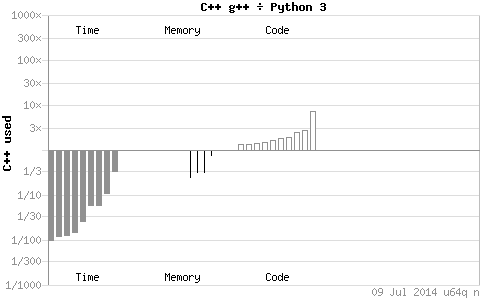
\includegraphics[width=0.8\textwidth]{img/cpp-py.png}
		\caption[\emph{Benchmark} entre \Cpp{} et \Python]{Étude de \emph{benchmark} entre \Cpp{} et \Python{}. Cette étude compare les performances de \Python{} par rapport au \Cpp{} en effectuant le quotient \fraction{Performance \Cpp}{Performance \Python}, donc les résultats en dessous de 1 sont en faveur de \Cpp{}, ceux au dessus de 1 en faveur de \Python{}. Les tests s'effectuent en 3 catégories, temps d'exécution, utilisation de la mémoire et nombre de lignes de code. Chaque barre de l'histogramme dans une catégorie correspond à un algorithme (\emph{n-body}, \emph{mendelbrot}, \emph{binary-trees}, etc.). Source : \url{http://benchmarksgame.alioth.debian.org/}}
		\label{fig:cpp-py}
	\end{figure}
\Python{} est certes moins performant que \Cpp{}, mais il a l'avantage de facilité la programmation avec un nombre de lignes de code moins élevé, des fonctions haut niveau dans la bibliothèque standard et l'interpréteur qui permet un débogage plus rapide. \Python{} est donc privilégié pour la partie interface ainsi que l'ordonnancement des différentes tâches, laissant le cœur du calcul à \Cpp{}.

%TODO: vérifier le choix définitif du SGBD, PostgreSQL permet d'effectuer plus facilement des requêtes en 2D, à vérifier par un petit benchmark.
		\paragraph{MySQL}
La partie base de données implique le choix d'un système de gestion de base de données (SGBD), celui-ci est MySQL. Ce choix est imposé par l'installation de ce logiciel dans l'environnement de développement qu'est le \CC{}.


% ----------------------------------------------------------------------
	\subsection{Outils de gestion de projet}
% ----------------------------------------------------------------------

Méthode kanban en ligne (chercher ou développer un outils pour, et proposer un accès à Bogdan).
% Il y a des outils en ligne gratuit pour faire du kanban mais je trouve pas ça aussi génial que sur papier. Trouver un truc cool pour pouvoir faire ça bien.

Diagramme de Gantt (pas le choix y'a Mouzat), permet planifier des tâches avec des "deadlines", d'affecter une tâche à une équipe, mais ici je suis seul à travailler sur le projet, un diagramme prévisionnel est disponible ici mais il est fortement hypothétique car je suis incapable de prévoir certains inprévu technique dû à mon statut d'externe au LPC. Je suis obligé de passer par certaines machines etc.


% ----------------------------------------------------------------------
% Méthode et résolution
% ----------------------------------------------------------------------
\part{Méthodes et résolution}
%%%%%%%%%%%%%%%%%%%%%%%%%%%%%%%%%%%%%%%%%%%%%%%%%%%%%%%%%%%%%%%%%%%%%%%%
% MÉTHODE ET RÉSOLUTION
%%%%%%%%%%%%%%%%%%%%%%%%%%%%%%%%%%%%%%%%%%%%%%%%%%%%%%%%%%%%%%%%%%%%%%%%


% ======================================================================
\section{Organisation des données}
% ======================================================================

% ----------------------------------------------------------------------
	\subsection{Détails des données}
% ----------------------------------------------------------------------

Nos données sont les résultats du \stack{} lors de la \DC{}, ainsi que les données de SDSS de la \emph{stripe 82} accessible depuis le Web. Ces données sont les résultats d'un traitement d'images captées par le télescope SDSS, il s'agit de sources lumineuses.

		\subsubsection{Définition d'un objet et d'une source}
% ^^^^^^^^^^^^^^^^^^^^^^^^^^^^^^^^^^^^^^^^^^^^^^^^^^^^^^^^^^^^^^^^^^^^^^

L'objet fait référence à l'astre que l'on observe dans le ciel dont données astrophysiques sont connus. Celles-ci inclus les coordonnées, la magnitude, la variation de la magnitude, ainsi que la parallaxe qui correspond au changement de coordonnées dû à la rotation de la Terre autour du Soleil.

La source quant à elle ne correspond qu'à l'image à un instant $t$ d'un objet. Les sources sont les éléments listés par le \stack{}, de même la base de données de SDSS est un catalogue de sources et non d'objets.

		\subsubsection{Impact sur les données}
% ^^^^^^^^^^^^^^^^^^^^^^^^^^^^^^^^^^^^^^^^^^^^^^^^^^^^^^^^^^^^^^^^^^^^^^

Les sources que nous analysons ont été observés à travers différents filtres allant de l'infra-rouge à l'ultra-violet, pour un total de 5 filtres. L'objet astrophysique est représenté à un instant $t$ par une source dans chaque filtre, l'association des sources entre les filtres a déjà été faite dans la base de données de SDSS, ce n'est pas le cas du \stack{}. Ainsi dans les données de SDSS nous retrouvons un calcul de magnitude apparente dans tous les filtres pour une source ; dans les données du \stack{} il y a une source différente par filtre, il y a donc un jeu de coordonnées par filtre.


% ----------------------------------------------------------------------
	\subsection{Modèles relationnels de la base de données}
% ----------------------------------------------------------------------

Deux modèles relationnels de la structure de la base de données ont été pensé. Le premier est un modèle classique et fiable, il s'agit du modèle dit « en étoile ». Le second est un modèle pensé pour optimiser le temps d'obtention des données de l'association, mais touche, à chaque ajout d'algorithme d'association, au modèle relationnel.

\ 

La base de données que nous souhaitons construire doit stocker à la fois les données nécessaire à l'analyse que nous allons effectuée (informations sur les sources du \stack{} et de SDSS), des données sur les différents algorithmes que nous allons utiliser ainsi que les résultats de ces algorithmes. Ces résultats étant l'association d'une source du \stack{} avec une source de SDSS.

		\subsubsection{Modèle en étoile}
% ^^^^^^^^^^^^^^^^^^^^^^^^^^^^^^^^^^^^^^^^^^^^^^^^^^^^^^^^^^^^^^^^^^^^^^

Il s'agit d'un modèle avec 4 tables. Tout d'abord deux tables pour stocker nos sources, une table pour les sources du \stack{} (\texttt{srcSTACK}) et une pour les sources de SDSS (\texttt{srcSDSS}). Ces tables sont crées et fixées lors de la récupération des données.

Une table est réservée pour les informations relatives aux algorithmes (\texttt{algorithms}) et contiendra des données comme le nom de l'algorithme, l'auteur, ainsi que la méthode utilisée par celui-ci, dans la pratique seul l'identifiant de l'algorithme nous intéressera.

Enfin les données relatives aux résultats de ces algorithmes sont tous stockés dans une même table (\texttt{matching}). Ces données sont associées à un identifiant unique, et contiennent l'identifiant de la sources du \stack{} que l'on associe et celui de la source de SDSS associée, mais aussi l'identifiant de l'algorithme utilisé.

Les informations sur ces tables est résumé dans la figure \ref{fig:bdd_star} sous la forme d'un diagramme.

	\begin{figure}[h]
		\centering
		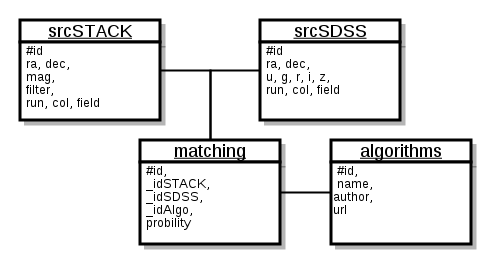
\includegraphics[width=0.9\textwidth]{img/bdd_star.png}
		\caption[Modèle relationnel en étoile]{Modèle relationnel en étoile pour stocker les sources identifiées par SDSS et le \stack{}, ainsi que les informations relatives aux algorithmes et l'association effectuée.}
		\label{fig:bdd_star}
	\end{figure}

Les deux tables contenant les sources ont une taille similaire $n$, par conséquent la table contenant les résultats de l'association contiendra $n$ données par nouvel algorithme si les algorithmes utilisés n'associent une source qu'à une seule source. Si un algorithme associe une source à plusieurs sources, ces données sont tout simplement stockées à l'aide de plusieurs identifiant unique dans notre base.


		\subsubsection{Modèle à colonnes variables}
% ^^^^^^^^^^^^^^^^^^^^^^^^^^^^^^^^^^^^^^^^^^^^^^^^^^^^^^^^^^^^^^^^^^^^^^
 
Il s'agit d'un modèle avec 3 tables. Comme précédement deux tables sont dédiées au stockage des sources, ainsi qu'une table pour les informations des algorithmes. Mais contrairement au modèle en étoile, on agit sur les deux tables contenant les sources en ajoutant une colonne par algorithme et en y stockant l'identifiant de la source associée. Ceci permet d'obtenir directement la liste des sources de l'autre base associées à une source.

Les informations sur ces tables est résumé dans la figure \ref{fig:bdd_colvar} sous la forme d'un diagramme.

	\begin{figure}[h]
		\centering
		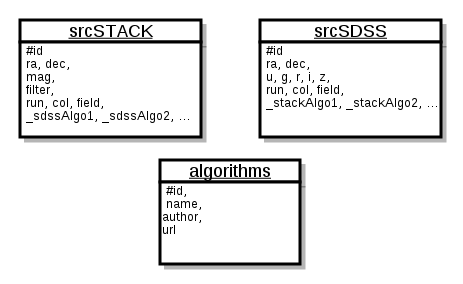
\includegraphics[width=0.9\textwidth]{img/bdd_colvar.png}
		\caption[Modèle relationnel à colonnes variables]{Modèle relationnel à nombre de colonnes variables pour stocker les sources identifiées par SDSS et le \stack{}, ainsi que les informations relatives aux algorithmes et l'association effectuée.}
		\label{fig:bdd_colvar}
	\end{figure}

Le problème est la modification du modèle relationnel qui peut entraîner une perte des données ou des lenteurs d'accès dû à l'ajout de données sur chaque ligne de la base.


% ======================================================================
\section{Jeu d'essai}
% ======================================================================

% ----------------------------------------------------------------------
	\subsection{Objectif}
% ----------------------------------------------------------------------

Il est courant d'effectuer des tests à partir de jeux d'essais, ceux-ci représente des cas standards d'utilisation ou permettent aussi de tester les limites d'un programme.

Dans notre cas le jeu d'essai est un ensemble de deux bases de données de sources. Une de ces bases est générée à partir de la première en ajoutant un bruit normal. Par conséquent chacune des sources à tester est généré à partir d'une de la base de référence, nos couples $(SDSS\,;\,Stack)$ sont prédéfinis. L'intérêt est donc de vérifier que nos algorithmes les associent correctement.

Après avoir fait tourner les programmes sur le jeu d'essai, nous meusurons trois quantités : les couples correctement formés, les couples erronés et les sources isolées. Il est important de maximiser la quantité des couples corrects. La quantité de minimiser en priorité est les couples erronés, il est préférable d'obtenir une absence d'information en obtenant une source seule plutôt qu'une mauvaise information.

\ 

À partir de ces résultats il est possible d'effectuer une ou plusieurs méthode d'optimisation en modifiant des paramètres d'entrée de nos algorithmes. La méthode la plus efficace est relativement simple à mettre en \oe{}uvre est la méthode du \emph{recuit-simulé}. L'absence de notion de voisinage dans le choix des paramètres complique l'utilisation d'une telle méthode car elle est conditionné par les tirages aléatoires des paramètres.

% ----------------------------------------------------------------------
	\subsection{Contrainte du jeu}
% ----------------------------------------------------------------------

Le jeu d'essai doit comporter certaines contraintes pour représenter au mieux la réalité. En effet il est possible qu'un programme associe plus facilement une source située en haut à gauche de la première, or si la génération aléatoire préconise ce placement, la détection d'un tel phénomène sera invisible. Il est donc important de posséder un bon générateur aléatoire.

En réalité en informatique il est très difficile d'avoir un générateur de nombres aléatoires (RNG pour \emph{random number generator}) puisque ces nombres sont issus d'un algorithme donc déterministes. On parle alors de générateurs de nombres pseudo-aléatoires (PRNG pour \emph{pseudo-random number generator}) car ces nombres sembles aléatoires. Une étude statistique permet de montrer que les générateurs de nombres pseudo-aléatoires possèdent une période et sont donc cycliques.

Le PRNG par défaut de \Cpp{} est considéré comme mauvais car ayant une courte période, sauf depuis \Cpp{}11 où un générateur plus performant a été implémenté. Ce nouveau générateur est l'algorithme de \emph{Mersenne Twister} découvert en 1997 et possédant une période de $2^{19937}-1$. Il est actuellement considéré comme un des meilleurs PRNG connu de par ses résultats au test de \emph{Diehard}, test des générateurs de nombres pseudo-aléatoires, et de par sa rapidité.

%% TODO: chercher une image montrant que certains PRNG sont mieux que d'autres

\ 

Il est aussi important de définir l'écart moyen et maximal prévu entre les données de SDSS et les résultats du \stack{} lors de la \DC{}. Le plus simple pour cela est d'utiliser les résultats déjà obtenu lors de mon précédent stage au LPC.

À partir de ces anciens résultats nous allons meusurer la largeur de la courbe en cloche obtenue, ainsi nous pouvons meusurer de façon empirique l'écart-type $\sigma$. Nous considèrerons que l'espérence est nulle. Ces deux informations permettent de définir une loi de probabilité normale $\mathcal{N}(\sigma,0)$. Cette loi de probabilité permet de créer un bruit gaussien sur les données de SDSS. Dans la pratique l'écart-type $\sigma$ est un vecteur de dimension 3, deux composantes pour l'ascension droite et la déclinaison, et une troisième pour la magnitude, obtenues à partir des mesures des écarts-types suivant ces trois paramètres.

	\begin{figure}[h]
		\centering
		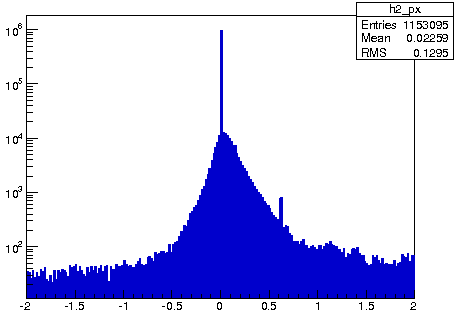
\includegraphics[width=0.9\textwidth]{img/mesuresigma.png}
		\caption[Mesure de l'écart-type à partir des anciens résultats]{Mesure de l'écart-type $\sigma$ à partir des résultats obtenus en août 2014.}
		\label{fig:mesuresigma}
	\end{figure}


% ======================================================================
\section{Recherche directe}
% ======================================================================

La première approche utilisée pour rechercher le plus proche voisin est une recherche dite diecte qui consiste à pour chaque point de la première base de données, on parcourt la seconde base, puis on compare le point de la première base et le point courant de la seconde.

	\begin{algorithm}
		\caption{Algorithme de recherche directe}
		\label{algo:direct-search}
		\begin{algorithmic}[1]
			\State $d_{min} \gets 100$; \Comment{Valeur arbitrairement grande de distance minimal d'initialisation}
			\For {$point_i$ dans la première base}
				\For {$point_j$ dans la deuxième base}
					\If {$d(point_i , point_j) < d_{min}$} \Comment{$d$ fonction de calcul de distance} \label{l:condi:algo:direct-search}
						\State $d_{min} \gets d(point_i , point_j)$;
					\EndIf
				\EndFor
			\EndFor
		\end{algorithmic}
	\end{algorithm}

Cet algoritme a une complexité en $\mathcal{O}(n^{2})$, il s'agit donc d'un algorithme relativement lent pour le problème à traiter, il n'est donc pas intéressant de l'utiliser sur un grand nombre de données. Malgré cela, cet algorithme est utilisé par sa modularité, en effet il est très simple de modifier la condition à la ligne \ref{l:condi:algo:direct-search} pour y prendre en compte la liste detous les paramètres que nous souhaitons prendre en compte.

\

L'optimisaton d'un tel algorithme peut se faire dans des cas particulier en effectuant un pré-traiement, d'une complexité parfois plus importante, permettant ensuite de réaliser un grand nombre de calcul rapidement. Il est donc nécessaire de trouver un juste milieu entre le temps d'éxécution du pré-traitement, et le gain obtenu par la suite au moment du traitement.

Il est aussi possible de lancer cette algorithme non pas sur toutes les données, mais sur un nombre restreint de données en découpant l'esapce en plusieurs morceaux. Cela équivaut à effectuer un partitionnement de l'espace.


% ======================================================================
\section[Arbres de partitionnement]{Structure d'arbres de partitionnement}
% ======================================================================

Certains algorithmes, ou approches algorithmiques, nécessite un partitionnement de l'espace des données pour diviser le travail et n'effectuer que des tâches élémentaires. Le pincipe de partition est proche d'une vision récursive, en effet on divise l'espace de travail tant que l'on ne se retrouve pas dans un cas simple que l'on sait traiter. Ceci permet de chercher le plus proche voisin mais aussi de créer des régions d'intéraction, cette dernière problématique ne nous intéressera pas ici. Le partitionnement est ensuite représenté par la structure d'un arbre comme une arborecense du partitionnement.

	\begin{figure}[h]
		\centering
		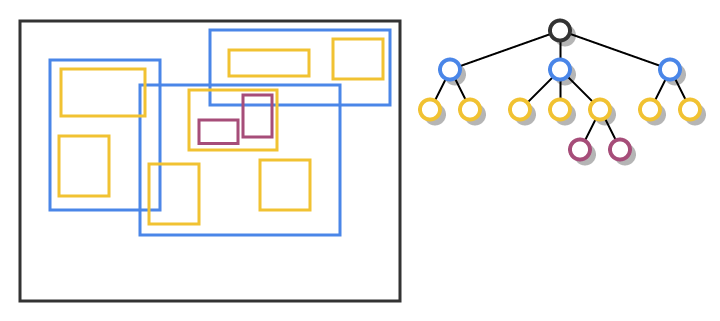
\includegraphics[width=0.9\textwidth]{img/rtree.png}
		\caption[Exemple de partitionnement et d'arbre associé]{Exemple d'arbre de partitionnement et de l'abre qui lui est assicié. Le principale intérêt est de travailler sur des ensembles de cardinal moins élevé, ou de mettre en valeur des espaces d'intéraction (\emph{R-tree} par exemple).}
	\end{figure}

Deux structures d'abre de partitionnement seront étudiées ici pour recherhcer le plus proche voisin, il s'agit du \emph{kd-tree} et du \emph{quad-tree}. Nous verrons les avantages et les inconvéniants des deux. Chaque n\oe{}ud de l'arbre représente une partition de l'espace, ses fils ses sous-partitions. Plusieurs partitionnements sont envisageables pour obtenir des divisons avec des propriétés plus ou moins intéressantes.


%-----------------------------------------------------------------------
	\subsection{Définition et propriété de l'espace de données}
%-----------------------------------------------------------------------

Avant de parler de l'algorithmie et des structures de données et il est important de parler des espaces dans lesquels nous allons travailler et de ce que nous voulons y faire. Les données que nous allons traiter sont des points dans un espace à 2 dimensions, et nous souhaitons rechercher le plus proche voisin. La définition du plus proche voisin n'est ici pas seulement d'ordre géométrique, en effet il est possible d'ajouter d'autres paramètres. La méthode choisi ici est dans un premier temps d'effectuer une discimination géométrique, puis le dernier choix selon d'autres critères.


Il est aussi possible de travailler en 3 dimensions, notre objectif est de travailler sur des sources lumineuses dans le ciel, par conséquent nous nous retrouvons avec deux dimensions d'espace (l'ascension droite et la déclinaison), mais il est aussi possible d'ajouter la magnitude (luminosité) comme dimension. Ainsi nous travaillerions dans un espace à 3 dimensions, dont 2 dimensions d'espace. Cette technique ne sera pas exploité ici car cela donne autant d'importance aux paramètres astrophysiques (ascension droite et déclinaison) qu'à un paramètre photométrique (magnitude) qui est fortement soumis aux erreurs de calibration et des conditions de mesure. Mathématiquement l'ajout de dimensions non spatiales (le temps ou un paramètre) n'est pas dérangeant et n'influe en rien la théorie. Ainsi il n'est pas rare de travailler en $n$ dimensions en fixant $n$ selon le besoin.

	\begin{figure}[h]
		\centering
			\subfloat[Espace à 2 dimensions.]{\label{fig:space2D}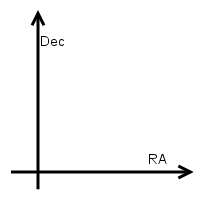
\includegraphics[height=4cm]{img/space2D.png}}
		\hspace{5pt}
			\subfloat[Espace à 3 dimensions.]{\label{fig:space3D}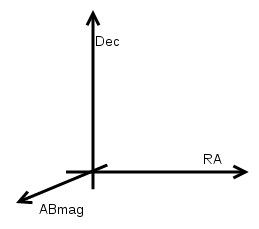
\includegraphics[height=4cm]{img/space3D.png}}
		\caption[Espace de travail à 2 ou 3 dimensions]{L'espace de travail peut être aussi bien à 2 qu'à 3 dimensions. L'exemple \ref{fig:space2D} montre un espace à 2 dimensions d'espaces ; l'exemple \ref{fig:space3D} montre un exemple d'espace à 2 dimensions d'espace et une de paramètres.}
		\label{fig:algoparsec}
	\end{figure}

\

La généralisation à $k$ dimensions est possible mais elle ne nous intéressera pas mais les différences des structures seront évoquées pour éveiller la curiosité du lecteur.

%-----------------------------------------------------------------------
	\subsection{Algorithme de construction}
%-----------------------------------------------------------------------

L'algorithme de construction de la structure du \emph{kd-tree} et du \emph{quad-tree} sont similaires, seule l'étape de division différe et est propre à chacune des structures. Le choix de la division implique des propriétés différentes sur les arbres générés. Cette étape sera détaillée en même temps que les différences des deux structures.

\

L'algorithme de construction est, sous sa forme la plus simple, récursif. Celui-ci est décrit dans l'algoritme \ref{algo:build-tree}.

	\begin{algorithm}
		\caption{Algorithme récursif de construction d'un arbre de partitionnement}
		\label{algo:build-tree}
		\begin{algorithmic}[1]
			\Function{Construire\_Arbre}{$espace$}
				\If{ nombre de points de l'espace = 0}
					\Comment{L'espace ne contient pas de source, impossible de diviser}
					\State \Return $espace$;
				\ElsIf{ nombre de point dans l'espace = 1}
					\Comment{L'espace ne contient plus qu'un point, il n'est plus nécessaire de diviser}
					\State \Return $espace$;
				\Else
					\Comment{Il faut diviser l'espace, et construire les sous espaces}
					\State \Return \Call{Construire\_Arbre}{ \textsc{Diviser\_Espace}($espace$) };
				\EndIf
			\EndFunction
		\end{algorithmic}
	\end{algorithm}

Le principe est simple, tant que l'espace contient plus d'une source on construit l'arbre sur les sub-divisions de l'espace. Quand il n'y a plus qu'une ou zéro source, on stope la division.


%-----------------------------------------------------------------------
	\subsection{Choix de la division}
%-----------------------------------------------------------------------

La différence entre la structure du \emph{quad-tree} et du \emph{kd-tree} est la méthode de divison de l'espace. Le partitionnement choisi possède des propriétés dépendante de cette méthode.

		\subsubsection{\emph{quad-tree}}
% ^^^^^^^^^^^^^^^^^^^^^^^^^^^^^^^^^^^^^^^^^^^^^^^^^^^^^^^^^^^^^^^^^^^^^^

La division du \emph{quad-tree} consiste à sub-diviser l'espace en quatre parties en prennant le milieu de chaque côté. Ceci permet de construire un arbre dont chaque n\oe{}ud possède 0 ou 4 fils.

La construction de cette arbre présente l'avantage d'être purement géométrique, ainsi il est possible d'effectuer un premier partitionnement pour utiliser un algorithme plus coûteux en complexité mais pouvant prendre en compte des paramètres plus fins d'association. En effet le plus proche voisin que nous cherchons n'est pas forcément le plus proche voisin géométrique mais le plus proche voisin en terme de ressemblance.

	\begin{figure}[h]
		\centering
		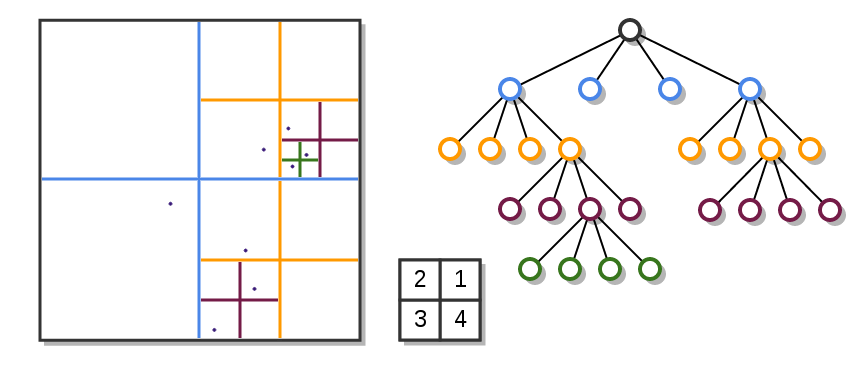
\includegraphics[width=0.9\textwidth]{img/quadtree.png}
		\caption[Relation entre la géométrie de l'ensemble et le \emph{quadtree} généré]{Relation entre la géométrie de l'ensemble (le placement des points dans l'espace), et la structure de données générée, le \emph{quadtree}. Chaque découpage est effectué avec une couleur différente pour voir son association avec l'arbre. La convention d'ordre des fils est celle des quadrants d'un repère orthonormé. On observe le découpage des sous-espaces tant qu'il n'y a pas zéro ou un élément.}
		\label{fig:quadtree}
	\end{figure}


Cette structure est généralisable facilement en 3 dimensions et portent le nom d'\emph{oct-tree}, chaque n\oe{}ud ne possède plus 4 mais 8 fils. Il est possible de passer en dimensions $k$ en divisant en 2 chaque axe, et ainsi obtenir $2^{k}$ sous-espace, donc $2^{k}$ fils à chaque n\oe{}ud.


Le problème de cette généralisation est la largeur et la profondeur de l'arbre obtenu, en effet si deux sources sont proches, il est parfois nécessaire d'effectuer un nombre important de divisions avant de réussir à séparer deux sources. C'est pour cette raison que cette algorithme ne sera utilisé que pour effectuer un premier partitionnement pour utiliser un algorithme plus lent sur des plus petites portions.


		\subsubsection{\emph{kd-tree}}
% ^^^^^^^^^^^^^^^^^^^^^^^^^^^^^^^^^^^^^^^^^^^^^^^^^^^^^^^^^^^^^^^^^^^^^^

La division du \emph{kd-tree} consiste à sub-diviser l'espace en tenant compte du nombre de points. En effet on remarque que le \emph{quad-tree} est très rarement équilibré, de nombreux n\oe{}uds ne servent pas, etc. Ces problèmes ont une cause commune qui est la division selon des critères géométriques sans tenir compte des données que l'espace contient. Ainsi la division du \emph{kd-tree} s'effectue suivant la médiane. Cette séparation permet d'obtenir deux sous-espaces contenant le même nombre de points plus ou moins 1 --- si l'espace contient un nombre impair de points.

Le problème de la médiane est que cette séparation s'effectue dans une liste, donc un espace à 1 dimension. La solution consiste à choisir à chaque itération une dimension selon laquelle nous effecturons la division. Ce choix s'effectue selon la parité de l'itération, si l'itération est pair nous effectuerons la division selon l'axe des $x$ (ascension droite dans notre cas), si l'itération est impair selon l'axe des $y$ (déclinaison).

	\begin{figure}[h]
		\centering
		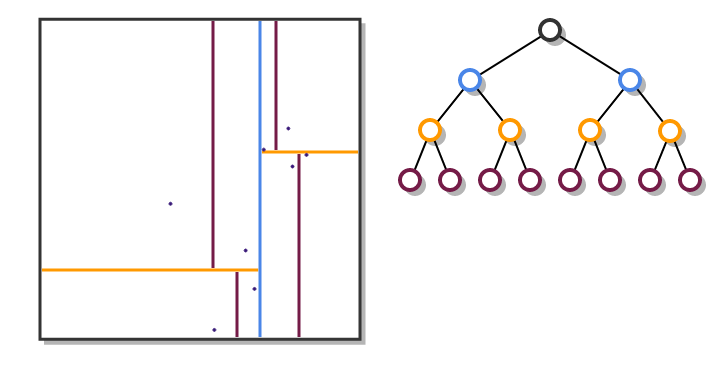
\includegraphics[width=0.9\textwidth]{img/kdtree.png}
		\caption[Relation entre la géométrie de l'ensemble et le \emph{kd-tree} généré]{Relation entre la géométrie de l'ensemble (le placement des points dans l'espace), et la structure de données générée, le \emph{kd-tree}. Chaque séparation divise l'espace en deux sous-espaces contenant un nombre égal de points. On remarque très facilement que l'arbre binaire est toujours équilibré grâce au découpage suivant la médiane.}
		\label{fig:kdtree}
	\end{figure}

Pour le cas de $k$ dimensions, le choix de la dimension s'effectue selon la congruence de l'itération modulo $k$, cela permet d'avoir une division régulière sur toutes les dimensions. La structure du \emph{kd-tree} évolue très bien au passage des dimensions supérieures puisqu'il s'agit toujours d'un arbre binaire dont la profondeur n'est que fonction du nombre de données. Quelque soit le nombre de dimensions la profondeur reste égale à $\log_{2}(n)$ où $n$ représente le nombre de points.



% ======================================================================
\section{Dérécursification}
% ======================================================================

L'algorithme \ref{algo:build-tree} est un algorithme dit récursif, cela signifie qu'il fait appelle à lui-même dans sa résolution. C'est le cas par exemple de la définition de la fonction factorielle.
	\begin{displaymath}
		\left\{\begin{tabular}{l}
			$n\,! = n \times (n-1)\,!$ \\
			$0\,!= 1$ \\
		\end{tabular}\right.
	\end{displaymath}
Lors de l'implémentation d'une telle fonction, celle-ci se rappelle elle-même jusqu'à un cas que l'on sait traiter c'est à dire factorielle de zéro. D'un point de vu informatique cela indique que nous ajoutons un appel de fonction dans la pile d'exécution. L'ajout d'information dans la pile d'exécution nuit à la performance mais aussi à la modularité du programme. Pour ces raisons il peut être intéressant de récursifier un algorithme. Cette technique revient à gérer soit même la pile d'exécution en ne sauvant pas tout l'appelle à la fonction mais seulement son résultat intermédiaire. Le résultat final est obtenu en dépilant les informations préalablement stockée dans la pile.


%-----------------------------------------------------------------------
	\subsection{Objectif}
%-----------------------------------------------------------------------

Notre algorithme est plus simple a comprendre sous sa forme récursive, et les seuls modifications que nous voulons apporter sont des limitations quant au nombre d'itérations. Ainsi l'aspect modulaire de la dérécursification ne nous intéresse pas, seul l'aspect performance nous intéresse.




% ----------------------------------------------------------------------
% Résultat et discussion
% ----------------------------------------------------------------------
\part{Résultats et discussion}
%%%%%%%%%%%%%%%%%%%%%%%%%%%%%%%%%%%%%%%%%%%%%%%%%%%%%%%%%%%%%%%%%%%%%%%%
% RÉSULTATS ET DISCUSSIONS
%%%%%%%%%%%%%%%%%%%%%%%%%%%%%%%%%%%%%%%%%%%%%%%%%%%%%%%%%%%%%%%%%%%%%%%%

% ======================================================================
\section{Base de données}
% ======================================================================

% ----------------------------------------------------------------------
	\subsection{Le retour client}
% ----------------------------------------------------------------------



% ----------------------------------------------------------------------
	\subsection{Efficacité}
% ----------------------------------------------------------------------

Étude de benchmark avec quelques requêtes régulièrement effectuée. Récupérer un csv avec les résultats et en sortir un joli boxplot avec R générer au moment de la compilation.

Voir fonction \texttt{BENCHMARK} de MySQL :
	\begin{verbatim}
		BENCHMARK(count,expr);
	\end{verbatim}
Le problème est que cette fonction ne permet d'être utilisé que sur des expression (\texttt{expr}) ne retournant qu'une ligne ou qu'une colonne.

% ----------------------------------------------------------------------
	\subsection{Maintenabilité}
% ----------------------------------------------------------------------

La base de données est documenté (voir annexe) donc c'est cool.


% ======================================================================
\section{Algorithmes de comparaison}
% ======================================================================

% ----------------------------------------------------------------------
	\subsection{Efficacité}
% ----------------------------------------------------------------------

		\subsubsection{Temps d'exécution}
% ^^^^^^^^^^^^^^^^^^^^^^^^^^^^^^^^^^^^^^^^^^^^^^^^^^^^^^^^^^^^^^^^^^^^^^

Utilisation de R pour la sortie (boxplot)


		\subsubsection{Utilisation mémoire}
% ^^^^^^^^^^^^^^^^^^^^^^^^^^^^^^^^^^^^^^^^^^^^^^^^^^^^^^^^^^^^^^^^^^^^^^

Utilisation de R pour la sortie (boxplot)


% ----------------------------------------------------------------------
	\subsection{Crédibilité du programme}
% ----------------------------------------------------------------------

Comparaison des vrais positifs, faux négatifs et vrais négatifs, faux positifs.


% ======================================================================
\section{Analyse des résultats}
% ======================================================================

% ----------------------------------------------------------------------
	\subsection{Résultat de la comparaison}
% ----------------------------------------------------------------------


% ----------------------------------------------------------------------
	\subsection{Conclusion sur le \emph{Stack}}
% ----------------------------------------------------------------------



%%% CONCLUSION %%%%%%%%%%%%%%%%%%%%%%%%%%%%%%%%%%%%%%%%%%%%%%%%%%%%%%%%%
\bookmarksetup{startatroot}
\addtocontents{toc}{\bigskip}
\newpage

\section{Conclusion}
%%%%%%%%%%%%%%%%%%%%%%%%%%%%%%%%%%%%%%%%%%%%%%%%%%%%%%%%%%%%%%%%%%%%%%%%
% CONCLUSION
%%%%%%%%%%%%%%%%%%%%%%%%%%%%%%%%%%%%%%%%%%%%%%%%%%%%%%%%%%%%%%%%%%%%%%%%

This is the end



%%% BIBLIOGRAPHY %%%%%%%%%%%%%%%%%%%%%%%%%%%%%%%%%%%%%%%%%%%%%%%%%%%%%%%
\newpage
\thispagestyle{plain}
\pagenumbering{alph}

\section*{Bibliographie \& Webographie}
\addcontentsline{toc}{section}{Bibliographie \& Webographie}
\nocite{*}
\bibliographystyle{alpha}
\bibliography{input/biblio}


%%% ANNEXES %%%%%%%%%%%%%%%%%%%%%%%%%%%%%%%%%%%%%%%%%%%%%%%%%%%%%%%%%%%%
%\appendix
%\newpage
%\pagenumbering{Roman}
%\part{Annexe}
%
%\section{Documentation des scripts et programmes réalisés}

\end{document}
